\documentclass[11pt,a4paper]{article}

% ── Encoding & fonts ──
\usepackage[utf8]{inputenc}
\usepackage[T1]{fontenc}
\usepackage{lmodern}

% ── Layout ──
\usepackage[margin=2.5cm]{geometry}
\usepackage{setspace}
\onehalfspacing

% ── Math ──
\usepackage{amsmath,amssymb,amsthm}

% ── Graphics & tables ──
\usepackage{graphicx}
\usepackage{float}
\usepackage{booktabs}
\usepackage{tabularx}
\usepackage{subcaption}

% ── References ──
\usepackage[authoryear,round]{natbib}

% ── Hyperlinks ──
\usepackage{hyperref}
\hypersetup{
    colorlinks  = true,
    linkcolor   = blue!60!black,
    citecolor   = blue!60!black,
    urlcolor    = blue!60!black,
}

% ── Appendix ──
\usepackage[toc,page]{appendix}

% ── Misc ──
\usepackage{enumitem}
\usepackage{caption}

% ══════════════════════════════════════════
%  TITLE
% ══════════════════════════════════════════
\title{Home Bias and International Risk Sharing:\\
       Empirical Replication and Extension}

\author{
    Philipp Cremer\thanks{Paris School of Economics.}
    \and Jannis Stagge\thanks{Paris School of Economics.}
    \and Felix Westerhoff\thanks{Paris School of Economics.}
}

\date{\today}

% ══════════════════════════════════════════
\begin{document}
\maketitle

\begin{abstract}
    % Write your abstract here.
    \noindent
    \textbf{Keywords:} home bias, risk sharing, equity portfolios, eurozone, financial integration \\
    \textbf{JEL Codes:} F36, F41, G11, G15
\end{abstract}

\newpage
\tableofcontents
\newpage

% ══════════════════════════════════════════
%  1  INTRODUCTION
% ══════════════════════════════════════════
\section{Introduction}\label{sec:introduction}

In their 2007 Paper Sørensen et al. argue that risk sharing and home bias, are two economic patterns 
that were analysed separately before but "may be manifestations of the same underlying
behavior". Home bias refers to the observation that investors hold disproportionally larger shares of domestic assets in their portfolio compared to theoretical predictions \cite{FrenchPoterba1991}.
Risk sharing denotes how countries stabilise their consumption or income from idiosyncratic output shocks via international financial markets \cite{Obstfeld1994}.
To analyse the potential link \textcite{main} use panel data for 24 OECD countries between 1993 and 2003. In their key regression,
they interact home bias measures with idiosyncratic GDP growth deviations in panel regressions of consumption and GNI growth. The results support their
hypothesis regarding the close connection of both phenomena showing that a decreasing home bias is statistically significant associated with increasing risk sharing without claiming causality.
With over 500 citations the paper has become an important reference linking portfolio allocation and risk sharing.

In this paper we replicate their main results, assess their robustness, and further extend their analytical framework by time and sample size\footnote{As much as possible,
constrained by data availability.} To deepen our understading of the empirical and economic relatonship between international financial integration
and macroeconomic risk sharing we shift our focus the Euro Area (EA) as case study. European Integration during the original papers sample period (1993--2003) 
and afterwards presents a fascinating opportunity to investigate, whether a decline in the exchange rate risk and 
transaction costs, two main reasons for home bias, is actually associated with a declining home bias and increasing risk sharing. 

Starting with the panel regression from \textcite{main}, our results are at odds with economic intuition. After relating it to findings in \textcite{main} for the European Union,
we thus disaggregate the analysis looking at home bias and risk sharing separately. The descriptive analysis of the EA's home bias trajectory creates new puzzles. Hence we turn to the literature,
finding that in fact, the data for the home bias construction in the EA is severely distorted from EU financial centers \cite{NBERw32275}. Due to data limitations we are not able
to construct corrected home bias measures. Thus we continue focussing on risk sharing. Because the risk sharing regressions do not provide sufficient
insights on diverging trajectoreis of the EA compared to comparable economies, nor on the relation to home bias we use a well established method to disentangle the different channels of risk sharing. Based on the hypothesized
connection between home bias and risk sharing, the capital markets channel of risk sharing should gain importance in the course of European integration.
Confirming this hypothesis we summarize the indicative evidence that indeed, with the introduction of the EA, home bias in the EA decreased stronger than in 
comparable countries while risk sharing increased.


% ══════════════════════════════════════════
%  2  DATA
% ══════════════════════════════════════════
\section{Data}\label{sec:data}



% ══════════════════════════════════════════
%  3  REPLICATION OF SØRENSEN ET AL. (2007)
% ══════════════════════════════════════════
\section{Replication of \textcite{sorensen2007}}\label{sec:replication}

\subsection{Equity Home Bias}\label{subsec:home_bias}

Based on data from the External Wealth of Nations Database \textcite{main} first report country-level foreign asset and liability holdings of equity, debt, and foreign direct investment 
relative to GDP for the 24 country sample. Using the same data from \texcite{lane2018external} we are able to replicate their Table 1 precisely with only minor deviations 
presumably due to data correction (see Table \ref{tab:table_1_repl} in Appendix \ref{app:replication}). In they following the establish a Home Bias measure.

Home bias conceptually builds on a standard Capital Asset Pricing Model (CAPM) implying that all investors hold equal shares of risky assets. Adapted to the country level, a country $i$ will
hold a share of domestic equity- (debt-) assets relative to the total portfolio equivalent to their world market share of equity- (debt-) assets. However, empirically domestic assets 
normally account for a higher proportion in the portfolio resulting in international home bias. Potential causes for home bias named in the literature are currency risk \cite{AdlerDumas1983}, 
transaction costs \cite{CooperKaplanis1994} as well as lack of information or market access.
\textcite{main} use a standard measure in the literature for the home bias. The index goes from 0 to 1 where 0 is international diversification in line with the CAPM prediction and 1 is full home bias. 
More specifically, they compute:

\begin{equation}
      \text{Equity Home Bias}_i = 1 - \frac{w_i^{\text{foreign}}}{1 - A_i}
\end{equation}

    where:

\begin{equation*}
      w_i^{\text{foreign}} = \frac{\text{Foreign equity held by country } i}{\text{Country } i\text{'s total equity portfolio}}
\end{equation*}

\begin{equation*}
      A_i = \frac{\text{Stock market capitalization of country } i}{\text{Stock market capitalization of the world}}
\end{equation*}

    and

\begin{equation*}
      \text{Total equity portfolio}_i = \text{Market cap}_i + \text{Foreign equity held}_i - \text{Domestic equity held by foreigners}_i
\end{equation*}

While the authors in our main replication paper compute an equity home bias and a debt home bias using the latter for robustness checks, we limit our analysis on the Equity Home Bias (EHB) due to data constraints. 
Closely following the paper we use data on equity holdings from \textcite{lane2018external}. Since the Standard and Poor Global Stock Markets Facebooks were not accessible for us, deviating from 
the original paper we used stock market capitalisation from the World Development Indicator Database by the World Bank which's coverage is fairly well for the 1993 to 2003 time period.
Using their methodology we can replicate columns (1) and (2) of their Table 2, descriptively showing percentage of foreign equity in portfolio (numerator of the EHB measure) and the EHB. The results align closely (see Table \ref{tab:table_2_rep} in Appendix \ref{app:replication}). 
Small deviations could come from data updates or the deviating source for stock market capitalisation. The EHB exhibits a consistent decline across countries from 1993 to 2003.

Next to some missing data points leading to missing EHB values for example for Ireland we excluded some observations. First, in few cases the total equity portfolio was negative leading to EHB values larger 1. 
Secondly, in even less cases EHB was negative which would be equivalent to a foreign bias. Both problems are most probably due to the data mismatch combining the EWN and WDI data. 
Problems arised in Finland from 1999 to 2003 potentially still related to the Finnish Banking crisis \cite{HonkapohjaKoskela1999} and in Italy, Austria and France for 1998 where each countries stock market capitalisation rapidly dropped 
before going back to the old level the next year. In 1998, both the Italian and the Austrian stock exchange was restructured or privatised potentially causing these data discontinuities \cite{WienerBoerse2026, BorsaItaliana2026}. Ireland had both, years with negative total equity or negative EHB. 
We completely discarded Ireland from the analysis. Potential explanations for this will be discussed in Section \ref{subsec:oofc}. 

Note that for the exploratory plots the original paper does not use the home bias measures but rather a rough proxy by looking at assets over GDP. This measure is also used for robustness checks. 
As can be seen in Appendix Table \ref{tab:table_1_repl} and Figure \ref{} we recover their results in trend and level.


\subsection{Cross-Section Risk Sharing}\label{subsec:replication_cs}

Recall that we are focussing our replication exercise on two main outputs. The first output plots (a scaled inverse of) cross-sectional risk-sharing estimates
against the (natural logarithm of) foreign assets over GDP (Figures 1 and 2 in \textcite{main}). It can be regarded as a graphical tool to analyze the co-movement
over time of year-by-year risk-sharing against a measure of financial openness which is likely inversely related to the Home Bias\footnote{The paper does not explain why 
it does not use the Home Bias measure previously described for its plots. We regard it to be a safety measure as the definition of the Equity Home Bias requires 
some more discretionary choice than simply using Foreign Assets over GDP and follow their approach exactly.}.\\
\indent For the cross-sectional risk-sharing regressions, we apply the methodology in \textcite[p.593]{main} which coincides with the standard approach in the literature. 
Specifically, we run regressions of the form:
\begin{equation}
    \Delta \log \mathrm{GNI}_{it}-\Delta \log \mathrm{GNI}_t = \text{constant} + \beta_{K,t}(\Delta \log \mathrm{GDP}_{it}-\Delta\log \mathrm{GDP}_t) + \varepsilon_{it},
\end{equation}
where $\mathrm{GNI}_{it}$ and $\mathrm{GDP}_{it}$ respectively measure Gross Domestic Income and Gross Domestic Product of country i at year t.
$\mathrm{GNI}_t$ and $\mathrm{GDP}_t$ denote the respective aggreagtes over the sample group at year t. Similarly, we run:
\begin{equation}
    \Delta \log \mathrm{C}_{it}-\Delta \log \mathrm{C}_t = \text{constant} + \beta_{C,t}(\Delta \log \mathrm{GDP}_{it}-\Delta\log \mathrm{GDP}_t) + \varepsilon_{it},
\end{equation}
where $\mathrm{C}$ denotes (aggregate or country-level) consumption.\\
\indent Just as in \textcite[p.21]{notes}, we may interpret $\beta_{j,t}=0, j\in\{C,K\}$ as the perfect risk-sharing benchmark. In this case,
idiosyncratic consumption growth perfectly tracks aggregate consumption growth and a country is fully insured against idiosyncratic output shocks.\\
\indent For completeness, we may conclude with the following remark. While consumers ultimately derive utility from consumption, equation (1) may be useful
in the context of this analysis because it relates more closely to the relationship under investigation. A decrease in the Home Bias manifests, ceteris paribus, in
higher net foreign factor factor income and therefore insulates consumption by insulating (gross) income. Running (1) may therefore provide a "better 'signal-to-noise' ratio"
\parencite[p. 589]{main}. It turns out that results are qualitatively similar which is why we focus on consumption risk sharing, and most often refer to the appendix for GNI risk sharing.\\

Turning to results, Figure \textbf{XXX} Panel A reproduces Figure 2 of the reference paper which is displayed in Panel B for easy comparability. It becomes apparent that we are able to
replicate the general trend proposed by \textcite{main}: Both the share of Foreign Assets and the amount of Risk Sharing increased in the 1990s for the chosen 
selection of 24 OECD countries, inspiring the more detailed Panel Regressions described in the next section.
For the Foreign Asset data, we near-perfectly reconstruct the yearly values. By contrast, the scaled cross-sectional risk-sharing estimates do not match the ones proposed in \textcite{main}. There are 
two possible reasons for this. First, it may be that our underlying GDP-, GNI and consumption data may be different from the authors' -- a possibility that we will discuss
at length in the next section. Second, note that \textcite{main} only show smoothed risk-sharing estimates "by using a Normal kernel with bandwidth (standard deviation) equal to 2" \parencite[p.594]{main}.
While we tried to get as close as possible to this smoothing technique, it would have been helpful had the authors provided their original estimates. Plotting them for our data, we find, in the words of the reference paper,
that the "year-by-year estimates fluctuate a fair amount" \textcite[p. 594]{main}, motivating the smoothing in the first place.\\
In conclusion, we regard the increasing trend in risk-sharing in the 1990s to be reliable, but are cautious about exact levels.
\begin{figure}[htbp]
    \centering
    % First subfigure
    \begin{subfigure}[b]{0.48\textwidth}
        \centering
        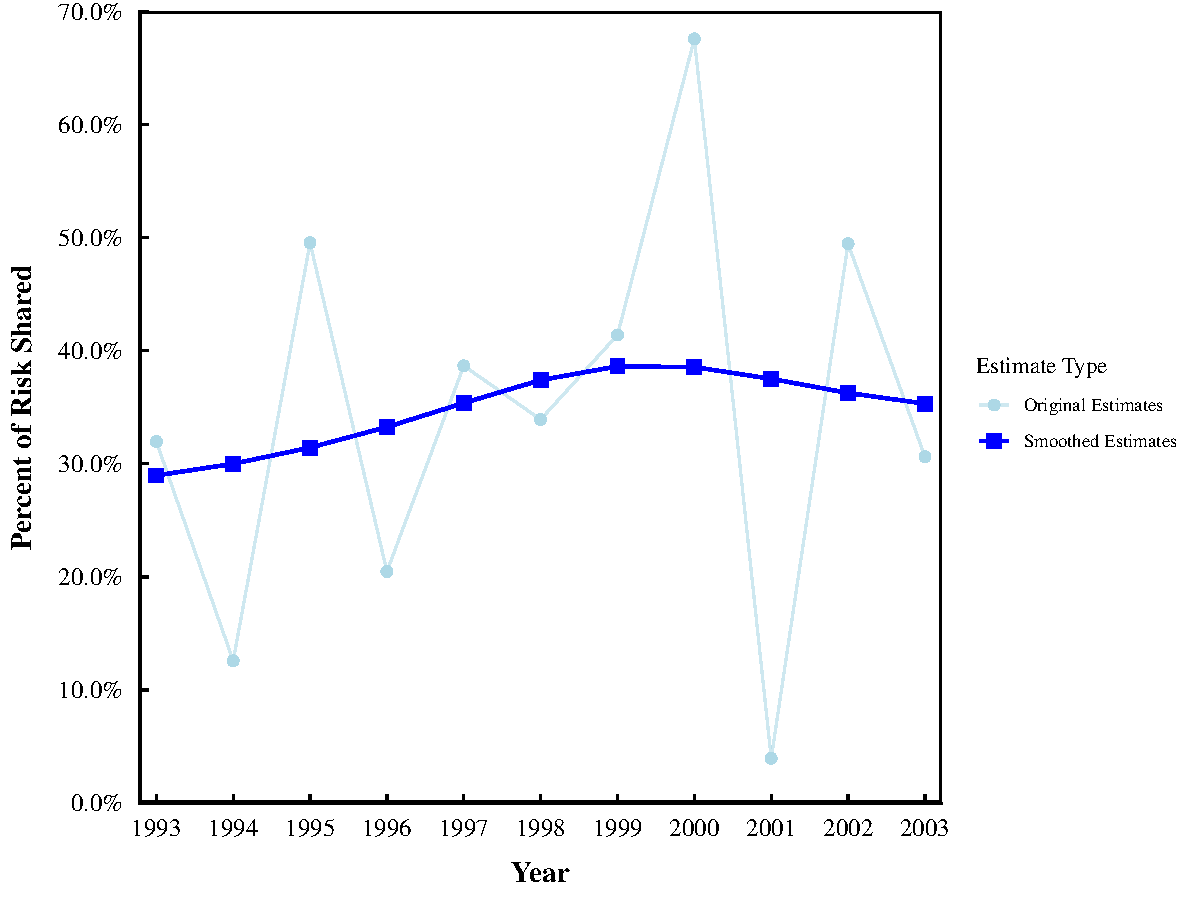
\includegraphics[width=\textwidth]{../output/rs_cs_rep_c.pdf}
        \caption{Replicated version}
    \end{subfigure}
    \hfill
    % Second subfigure
    \begin{subfigure}[b]{0.48\textwidth}
        \centering
        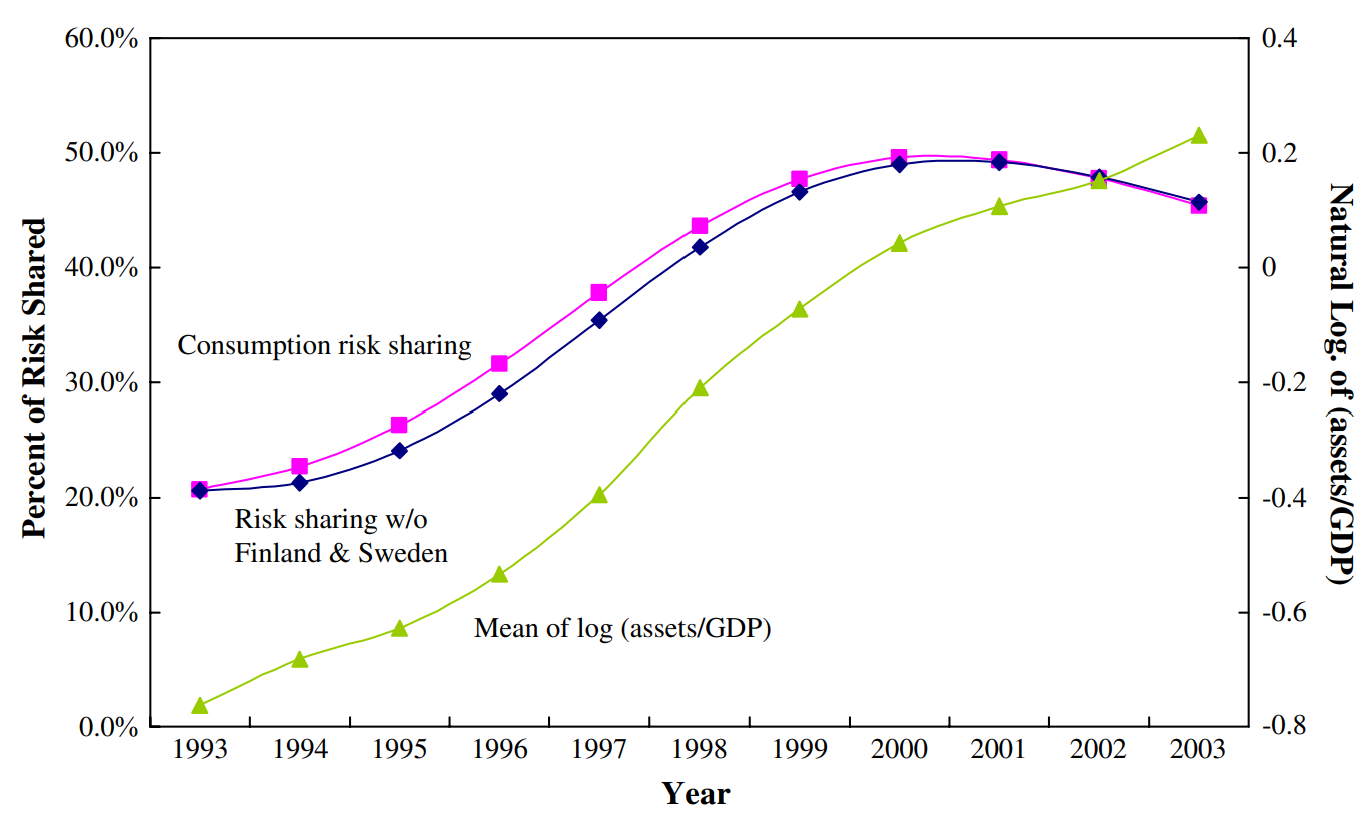
\includegraphics[width=\textwidth]{../output/main_fig_2.png}
        \caption{Original Paper}
    \end{subfigure}
    \hfill    
    \caption{Consumption Risk Sharing and foreign asset holdings}
\end{figure}

\subsection{Panel-Data Regressions}\label{subsec:replication_panel}

\subsubsection{Theoretical outline}

\textcite{main} use a panel regression framework to analyse whether a lower equity home bias is associated with a higher degree of income risk
sharing and consumption risk sharing. To do so, they regress the log growth rate of
country-specific Gross National Income (GNI) or consumption (C), relative to the
sample-wide log growth rate of GNI or consumption, on the country-specific log growth
rate of Gross Domestic Product (GDP), relative to the sample-wide log growth rate of
GDP. The baseline regression is

\begin{equation}
\Delta \log C_{it} - \Delta \log C_t
=
\alpha_i
+
\kappa
\left(
\Delta \log GDP_{it} - \Delta \log GDP_t
\right)
+
\epsilon_{it}.
\end{equation}

As in the cross-sectional regressions, one minus the respective coefficients
\(\kappa\) measures the average degree of risk sharing. A lower
coefficient therefore corresponds to a higher degree of risk sharing.

To incorporate equity home bias into the panel regression, the authors allow the
coefficient on relative GDP growth to vary with both a time trend and the deviation of
a country's equity home bias from the sample average:

\begin{equation}
\kappa
=
\kappa_0
+
\kappa_1(t - \overline{t})
+
\kappa_2(EHB_{it} - \overline{EHB}_t)
\end{equation}


It is therefore most intuitive to interpret the implied degree of risk sharing
directly. 

and for consumption risk sharing by

\begin{equation}
CRS_{it}
=
1 - \kappa_0
-
\kappa_1(t - \overline{t})
-
\kappa_2(EHB_{it} - \overline{EHB}_t).
\end{equation}

where \(CRS_{it}\) stand for income and consumption risk sharing. Similarly, they run the above regression 
with GNI plugged in for consumption.\footnote{See \textcite{main} for a more extensive discussion. For the sake of simplicity, we decided to present only the consumption regression.
In the tables below, both regression results are reported.}
For the hypothesis of a potential co-movement between equity home bias and risk
sharing, the main coefficient of interest is therefore \(-\kappa_2\). A positive value of \(\kappa_2\) implies that a higher equity home bias
increases the sensitivity of relative consumption growth to relative GDP growth and therefore
reduces consumption risk sharing. Equivalently, an increase in equity home bias by 0.1
changes consumption risk sharing by \(-0.1\kappa_2\).
All panel regressions are estimated using a two-stage feasible GLS-type approach.
In the second-stage regression, each country is assigned a weight proportional to one over the
 the standard error of its first-stage residuals.\footnote{Since this
procedure is weakly documented in the original paper, we compared the first- and
second-stage regression results. The differences do not affect the direction or
statistical significance of the main coefficients.}

\subsubsection{Empirical results}
When reporting the results of the panel regressions, we follow
the authors standard and report the easier to interpret 
coefficients \(1-\kappa_0\), \(-\kappa_1\) and \(-\kappa_2\) multiplied
by 100 to interpret them as percentage effects. Our panel regression results follow the key results of 
\textcite{main},with a statistically 
non-different to zero estimate for the time trend and a highly significant coefficient
for the equity home bias both on income and consumption risk sharing. An increase in the equity home bias by 0.1 
is now associated with an increase in income risk sharing by roughly 13 percent and consumption risk sharing by 
roughly 20 percent. Given that our point estimates for the coefficient are larger than 100 and 
notably higher than the point estimates found by \textcite{main}, we believe that the discussed data choices, aswell as data revisions and the choice of the 
base year play an important role. Further, we rely on an interpretation
offered by the authors themseves, believing that a coefficient of more than 100 percent risk sharing likely indicates a strong co-movement, even if the point estimate is not likely to 
hold in larger samples.\footnote{A statement that proves to be true once we extend the sample period from 1993--2003 to 1987--2017.} Our coefficient for average income risk sharing
is highly significant, while it is not in the original paper. Given that it will turn non-significant in the larger sample period, we observe this, but doubt that it affects the main 
findings of this exercise. 

\begin{table}[!htbp] 
\centering 
\caption{Income and Consumption Risk Sharing and Equity Home Bias: OECD 1993--2003} 
\label{tab:risk_sharing_ehb_oecd} 

\begin{tabular}{@{\extracolsep{5pt}}lccc} 
\\[-1.8ex]\hline 
\hline \\[-1.8ex] 
 & Average Risk Sharing & Time Trend & Equity Home Bias \\ 
\hline \\[-1.8ex] 

Income 
& 16 
& 1 
& $-$133 \\ 
& (4.16) 
& (0.76) 
& (4.87) \\ 

Consumption 
& 55 
& 1 
& $-$204 \\ 
& (15.10) 
& (0.52) 
& (9.07) \\ 

\hline 
\hline \\[-1.8ex] 
\end{tabular} 

\vspace{0.15cm}

\begin{minipage}{\linewidth}
\footnotesize
\textit{Note:} Values in parentheses are absolute t-values. Replication sample with 22 OECD countries included in the panel regression in table 3 of the original paper. The income and consumption row present \(100 \cdot (1-\kappa_0)\), \(100 \cdot (-\kappa_1)\), and \(100 \cdot (-\kappa_2)\). Country-fixed effects included.
\end{minipage}

\end{table}

Running the same regressions on foreign asset holdings over GDP, as done by \textcite{main} confirms the robustness of our replication exercise. Even 
though we find party differing point estimates, the direction and significance of the point estimates are in line with the original paper.\footnote{Note that a positive 
sign of \(-\kappa_2\) is now associated with a higher level of risk sharing.}  We treat these regressions as an robustness check and find posiive \(-\kappa_2\) coefficients 
for all forms of asset holdings, and statistically non signfiicant estimates for the time trend.

Leading us to conclude that the main findings of \textcite{main} panel regressions can be replicated with updated data two decades later.
We treat these regressions merely as an robustness check, and find postive \\

\begin{table}[!htbp] 
\centering 
\caption{Risk Sharing and Foreign Asset Holdings Relative to GDP: OECD 1993--2003} 
\label{tab:asset_holdings_oecd} 

\scriptsize
\setlength{\tabcolsep}{3pt}
\renewcommand{\arraystretch}{1.15}

\resizebox{\linewidth}{!}{%
\begin{tabular}{lccccccc}
\hline 
\hline \\[-1.8ex]

\begin{tabular}{@{}l@{}}With country-fixed\\effects\end{tabular}
& \begin{tabular}{@{}c@{}}Average risk\\sharing\end{tabular}
& \multicolumn{6}{c}{Interaction terms with GDP} \\
\cline{3-8}
\\[-1.8ex]
& 
& Trend 
& Equity 
& Debt 
& FDI 
& Equity + Debt 
& All Assets \\

\hline \\[-1.8ex]

\begin{tabular}{@{}l@{}}Income risk\\sharing\end{tabular}
& 15 (4.15) 
& 1 (1.21) 
& 12 (5.19) 
& 
& 
& 
& \\

& 16 (4.21) 
& 1 (0.72) 
& 
& 18 (5.15) 
& 
& 
& \\

& 10 (2.79) 
& 2 (1.63) 
& 
& 
& 12 (3.33) 
& 
& \\

& 16 (4.25) 
& 1 (0.73) 
& 
& 
& 
& 18 (5.05) 
& \\

& 16 (4.26) 
& 1 (1.06) 
& 
& 
& 
& 
& 21 (5.14) \\

\\[-0.5ex]

\begin{tabular}{@{}l@{}}Consumption\\risk sharing\end{tabular}
& 57 (14.77) 
& 1 (0.90) 
& 18 (8.80) 
& 
& 
& 
& \\

& 50 (12.16) 
& 0 (0.15) 
& 
& 21 (6.01) 
& 
& 
& \\

& 52 (12.59) 
& 0 (0.41) 
& 
& 
& 14 (6.16) 
& 
& \\

& 52 (12.93) 
& 0 (0.32) 
& 
& 
& 
& 23 (6.81) 
& \\

& 55 (13.59) 
& 0 (0.46) 
& 
& 
& 
& 
& 24 (7.35) \\

\hline 
\hline
\end{tabular}%
}

\vspace{0.15cm}

\begin{minipage}{\linewidth}
\footnotesize
\textit{Note:} Values in parentheses are absolute t-values. Replication sample with 22 OECD countries included in the panel regression in table 3 of the original paper. For income and consumption risk sharing, the reported coefficients are \(100 \cdot (1-\kappa_0)\), \(100 \cdot (-\kappa_1)\), and \(100 \cdot (-\kappa_2)\). Country-fixed effects included.
\end{minipage}

\end{table}


% ══════════════════════════════════════════
%  4  EXTENSIONS WITHIN THE ORIGINAL FRAMEWORK
% ══════════════════════════════════════════
\section{Extensions by Time and Sample Size}\label{sec:extensions_time}

As a logical extension and robustness check of the results in \textcite{main} we apply the entire methodology to a longer sample with the original countries and 
additionally a longer sample with broader country coverage. The time period and country sample chosen was partly defined by data restrictions for the EHB as desrcibed in the following.

\subsection{Extension: Equity Home Bias}\label{subsec:ext_home_bias}

For the time and country coverage extension the methodology for the home bias remains the same. Due to limited data coverage before the 1980s we decided to start the series in 1987, five years before the Maastricht Treaty. 
In the second half of the 2010s the WDI world market capitalisation is less complete especially for EU countries. Hence, we limited the long sample to 2017 also considering potential irregular patterns during Covid and Ukraine crisis. 
For the broader country sample to address the coverage we first limited the data to the joint subset of the top 50 economies based on the EWN reported GDP values combined with all EU27 countries. 
Starting from there we analysed irregularities in the EHB index as before (excluding e.g. Luxembourg and Ireland due to negative total equity portfolio values).
Because the regression uses deviations from the mean we tried to avoid frequent drop ins or outs. Instead of keeping countries with very few non NA values for EHB, we eventually excluded Ireland, 
Luxembourg, Finland, Malta, Cyprus, Lithuania, Latvia and Estonia as well as Taiwan from the broader sample. All remaining countries in the broad sample have an EHB coverage of at least 40\%. 
For a visual analysis of the data coverage after excluding irregular observations see Figure \ref{fig:app_cover_ehb} in Appenix \ref{app:rep_ext}.


\subsection{Extension: Cross-Section Risk Sharing Estimates}\label{subsec:ext_replication_cs}

\subsection{Extension: Panel-Data Regressions}\label{subsec:ext_replication_panel}

% ============================================================
\subsubsection{First Extension: Similar Country Sample 1987--2017}
% ============================================================
By keeping the original sample of 22 OECD countries and extending the observation period by 20 years to 1987--2017 we aim to analyse whether the authors findings 
are robust on a longer time horizon, as the original sample period of 11 years is rather short. 

FELIX TEIL: CROSS SECTION:Looking at figure (XXX), we can see that the cross section risk sharing coefficient has increased constantly from 1987
to 2000, using the same smoothing method as the authors in the paper. After a short dip during 2000 to 2003, potentially caused
by the \textit{dotcom}-bubble, we observe an even stronger increase in cross section risk sharing that is ended apruptly by the 
global financial crisis 2007/2008. After this crisis, global cross section risk sharing grows even stronger. 
Looking at the curve for foreign assets over GDP we can see that they constantly increased over the time period of 31 years. 

Panel regressions find that the main relationship between Equity Home Bias and risk sharing largely hold when extending the 
time period by 20 years. A 0.1 decrease of the equity home bias is now associated with a roughtly 3 percent increase 
in income risk sharing and a 8 percent increase in consumption risk sharing. The average risk sharing coefficient decreases notably, and becomes 
statistically non-significant for income risk sharing. Given that this coefficient was non significant in \textcite{main} for the original sample period, 
it seems to be a parameter that varies, depending on sample and data. Most relevant is the signficance of \(-\kappa_2\). /
Focusing on the foreign asset over GDP regressions gives robustness to conclude that the negative relationship between Home Bias and risk sharing holds over the extended time period.
conclude that the negative relationship between Home Bias and Income and Consumption Risk sharing holds for the extended period.

\begin{table}[!htbp] 
\centering 
\caption{Income and Consumption Risk Sharing and Equity Home Bias: OECD 1987--2017} 
\label{tab:risk_sharing_ehb_extended} 

\begin{tabular}{@{\extracolsep{5pt}}lccc} 
\\[-1.8ex]\hline 
\hline \\[-1.8ex] 
 & Average Risk Sharing & Time Trend & Equity Home Bias \\ 
\hline \\[-1.8ex] 

Income 
& 0 
& 0 
& $-$28 \\ 
& (0.14) 
& (0.82) 
& (2.80) \\ 

Consumption 
& 40 
& 0 
& $-$81 \\ 
& (19.61) 
& (0.29) 
& (7.96) \\ 

\hline 
\hline \\[-1.8ex] 
\end{tabular} 

\vspace{0.15cm}

\begin{minipage}{\linewidth}
\footnotesize
\textit{Note:} Values in parentheses are absolute t-values. Replication sample with 22 OECD countries included in the panel regression in table 3 of the original paper. Extended time period 1987--2017 For income and consumption risk sharing, the reported coefficients are \(100 \cdot (1-\kappa_0)\), \(100 \cdot (-\kappa_1)\), and \(100 \cdot (-\kappa_2)\). Country-fixed effects included.
\end{minipage}

\end{table}
\begin{table}[!htbp] 
\centering 
\caption{Risk Sharing and Foreign Asset Holdings Relative to GDP: OECD 1987--2017} 
\label{tab:asset_holdings_extended} 

\scriptsize
\setlength{\tabcolsep}{3pt}
\renewcommand{\arraystretch}{1.15}

\resizebox{\linewidth}{!}{%
\begin{tabular}{lccccccc}
\hline 
\hline \\[-1.8ex]

\begin{tabular}{@{}l@{}}With country-fixed\\effects\end{tabular}
& \begin{tabular}{@{}c@{}}Average risk\\sharing\end{tabular}
& \multicolumn{6}{c}{Interaction terms with GDP} \\
\cline{3-8}
\\[-1.8ex]
& 
& Trend 
& Equity 
& Debt 
& FDI 
& Equity + Debt 
& All Assets \\

\hline \\[-1.8ex]

\begin{tabular}{@{}l@{}}Income risk\\sharing\end{tabular}
& $-$2 (0.87) 
& 0 (0.70) 
& 5 (3.59) 
& 
& 
& 
& \\

& 0 (0.21) 
& 0 (0.80) 
& 
& 8 (4.14) 
& 
& 
& \\

& $-$2 (0.98) 
& 0 (0.40) 
& 
& 
& 4 (2.57) 
& 
& \\

& $-$1 (0.62) 
& 0 (0.91) 
& 
& 
& 
& 8 (4.15) 
& \\

& $-$2 (1.03) 
& 0 (0.74) 
& 
& 
& 
& 
& 8 (4.08) \\

\\[-0.5ex]

\begin{tabular}{@{}l@{}}Consumption\\risk sharing\end{tabular}
& 42 (20.31) 
& 0 (0.28) 
& 10 (9.07) 
& 
& 
& 
& \\

& 39 (18.10) 
& 0 (0.72) 
& 
& 12 (5.60) 
& 
& 
& \\

& 40 (19.21) 
& 0 (0.18) 
& 
& 
& 11 (7.41) 
& 
& \\

& 40 (18.98) 
& 0 (0.58) 
& 
& 
& 
& 14 (7.06) 
& \\

& 41 (19.35) 
& 0 (0.40) 
& 
& 
& 
& 
& 15 (7.60) \\

\hline 
\hline
\end{tabular}%
}

\vspace{0.15cm}

\begin{minipage}{\linewidth}
\footnotesize
\textit{Note:} Values in parentheses are absolute t-values. Original sample and extended time period. For income risk sharing, the reported coefficients are \(100 \cdot (1-\kappa_0)\), \(100 \cdot (-\kappa_1)\), and \(100 \cdot (-\kappa_2)\). For consumption risk sharing, the reported coefficients are \(100 \cdot (1-\eta_0)\), \(100 \cdot (-\eta_1)\), and \(100 \cdot (-\eta_2)\). Country-fixed effects included.
\end{minipage}

\end{table}
% ============================================================
\subsubsection{Second Extension: Extended Country Sample 1987--2017}
% ============================================================
Extending the OECD sampe to 29 countries
\footnote{For the GNI analysis and panel regressions some observations drop, due to a lack of data coverage for both Consumption, GNI, GDP 
and the Equity Home Bias. A future extention of \textcite{main} should certainly try extend the country sample beyond OECD countries. Due to our data problems, we decided to keep a rather
small, but consistent sample.} for the sample period 1987--2017 gives us the opportunity to analyse if the main findings of \textcite{main} can be 
extended to a broader set of countries. As a potential shortcoming of this extention, we must admit that the sample size is still rather small. 
The panel-regression results of the (slightly) extended sample between 1987 and 2017 confirm the same results as shown in the 
two regressions before. 
An decrease in the Equity Home Bias by 0.1 is associated with an increase of income risk sharing by roughly 3 percent and
an increase in consumption risk sharing by roughly 8 percent. 


Again, the panel regressions for foreign Asset holdings relative to GDP confirm this estimation, with highly significant estimations 
for the asset holdings themselves, and non significant estimations for the time trend. Again, the average risk sharing coefficient for 
income is non significant in both specifications, while it is highly significant for consumption in both specifications.

\begin{table}[!htbp] 
\centering 
\caption{Income and Consumption Risk Sharing and Equity Home Bias: Extended OECD Sample 19987--2017} 
\label{tab:risk_sharing_ehb_extended_sample} 

\begin{tabular}{@{\extracolsep{5pt}}lccc} 
\\[-1.8ex]\hline 
\hline \\[-1.8ex] 
 & Average Risk Sharing & Time Trend & Equity Home Bias \\ 
\hline \\[-1.8ex] 

Income 
& 0 
& 0 
& $-$28 \\ 
& (0.34) 
& (0.26) 
& (3.24) \\ 

Consumption 
& 30 
& 0 
& $-$84 \\ 
& (15.28) 
& (0.41) 
& (8.25) \\ 

\hline 
\hline \\[-1.8ex] 
\end{tabular} 

\vspace{0.15cm}

\begin{minipage}{\linewidth}
\footnotesize
\textit{Note:} Values in parentheses are absolute t-values. Extended sample with up to 29 OECD countries, many observations lost due to missing data coverage. Extended time period 1987--2017. For income and consumption risk sharing, the reported coefficients are \(100 \cdot (1-\kappa_0)\), \(100 \cdot (-\kappa_1)\), and \(100 \cdot (-\kappa_2)\). Country-fixed effects included.
\end{minipage}

\end{table}
\begin{table}[!htbp] 
\centering 
\caption{Risk Sharing and Foreign Asset Holdings Relative to GDP: Extended OECD Sample and 1987--2017} 
\label{tab:asset_holdings_extended_sample} 

\scriptsize
\setlength{\tabcolsep}{3pt}
\renewcommand{\arraystretch}{1.15}

\resizebox{\linewidth}{!}{%
\begin{tabular}{lccccccc}
\hline 
\hline \\[-1.8ex]

\begin{tabular}{@{}l@{}}With country-fixed\\effects\end{tabular}
& \begin{tabular}{@{}c@{}}Average risk\\sharing\end{tabular}
& \multicolumn{6}{c}{Interaction terms with GDP} \\
\cline{3-8}
\\[-1.8ex]
& 
& Trend 
& Equity 
& Debt 
& FDI 
& Equity + Debt 
& All Assets \\

\hline \\[-1.8ex]

\begin{tabular}{@{}l@{}}Income risk\\sharing\end{tabular}
& 1 (0.63) 
& 0 (0.68) 
& 3 (3.40) 
& 
& 
& 
& \\

& 0 (0.20) 
& 0 (0.93) 
& 
& 7 (4.72) 
& 
& 
& \\

& $-$2 (1.23) 
& 0 (0.62) 
& 
& 
& 4 (3.23) 
& 
& \\

& 0 (0.05) 
& 0 (1.09) 
& 
& 
& 
& 7 (4.65) 
& \\

& 0 (0.27) 
& 0 (0.94) 
& 
& 
& 
& 
& 7 (4.54) \\

\\[-0.5ex]

\begin{tabular}{@{}l@{}}Consumption\\risk sharing\end{tabular}
& 28 (14.42) 
& 0 (0.56) 
& 12 (11.26) 
& 
& 
& 
& \\

& 30 (14.02) 
& 0 (0.49) 
& 
& 10 (4.75) 
& 
& 
& \\

& 26 (11.85) 
& 0 (2.00) 
& 
& 
& 12 (7.78) 
& 
& \\

& 28 (13.53) 
& 0 (0.00) 
& 
& 
& 
& 13 (6.73) 
& \\

& 28 (13.46) 
& 0 (0.27) 
& 
& 
& 
& 
& 14 (7.37) \\

\hline 
\hline
\end{tabular}%
}

\vspace{0.15cm}

\begin{minipage}{\linewidth}
\footnotesize
\textit{Note:} Values in parentheses are absolute t-values. Extended sample with up to 29 OECD countries, many observations lost due to missing data coverage. Extended time period 1987--2017. For income and consumption risk sharing, the reported coefficients are \(100 \cdot (1-\kappa_0)\), \(100 \cdot (-\kappa_1)\), and \(100 \cdot (-\kappa_2)\). Country-fixed effects included.
\end{minipage}

\end{table}


% ══════════════════════════════════════════
%  5  EUROZONE EXTENSION
% ══════════════════════════════════════════
\section{Case Study Euro Area}\label{sec:euro_case}

As our main extension, we examine the EA as a case study. The introduction of the euro eliminated exchange rate risk among member states and, fueled by further European Integration, 
transaction costs for cross border financial flows fell. As introduced in Section \ref{subsec:home_bias} those are commonly seen as drivers of home bias.
The EA therefore provides a setting where we would expect a pronounced decline in home bias compared to similar countries. Following the established association, risk sharing should increase correspondingly.
Based on our longer sample we can leverage a considerably long period of EA integration and expansion.

\subsection{Case Study Euro Area: Panel Regression}

Using the EA as its own sample leads to rather unintuitive results, both on a cross section and panel regression level. As can be seen in the following two tables, the point 
estimates are notably smaller than for the OECD sample and the coefficient for the Equity Home Bias on consumption is not significant anymore. 
\textcite{main} note the same puzzling irregularities when looking at an EU sample, especially with respect to the Consumption risk sharing coefficient among EU countries. They cite 
(XXX) and speculate that consumption risk sharing within the EU has decreased due to less-pro cyclical government spending among EU countries due to the Maastricht criteria. We 
understand that this reasoning can be applied to the EA aswell and tried to run structural break regressions to understand this relationship further. Due non robustly significant results 
in those structural break regressions, we shift our focus to a different set of tools to analyse the relationship further. 

\begin{table}[!htbp] 
\centering 
\caption{Income and Consumption Risk Sharing and Equity Home Bias: Euroarea 1987--2017} 
\label{tab:risk_sharing_ehb_euroarea} 

\begin{tabular}{@{\extracolsep{5pt}}lccc} 
\\[-1.8ex]\hline 
\hline \\[-1.8ex] 
 & Average Risk Sharing & Time Trend & Equity Home Bias \\ 
\hline \\[-1.8ex] 

Income 
& 0 
& 0 
& $-$30 \\ 
& (0.09) 
& (0.96) 
& (2.16) \\ 

Consumption 
& 27 
& $-$1 
& $-$8 \\ 
& (8.85) 
& (3.48) 
& (0.50) \\ 

\hline 
\hline \\[-1.8ex] 
\end{tabular} 

\vspace{0.15cm}

\begin{minipage}{\linewidth}
\footnotesize
\textit{Note:} Values in parentheses are absolute t-values. Euroarea sample for the period 1987--2017. For income and consumption risk sharing, the reported coefficients are \(100 \cdot (1-\kappa_0)\), \(100 \cdot (-\kappa_1)\), and \(100 \cdot (-\kappa_2)\). Country-fixed effects included.
\end{minipage}

\end{table}
\begin{table}[!htbp] 
\centering 
\caption{Risk Sharing and Foreign Asset Holdings Relative to GDP: Euroarea 1987--2017} 
\label{tab:asset_holdings_euroarea} 

\scriptsize
\setlength{\tabcolsep}{3pt}
\renewcommand{\arraystretch}{1.15}

\resizebox{\linewidth}{!}{%
\begin{tabular}{lccccccc}
\hline 
\hline \\[-1.8ex]

\begin{tabular}{@{}l@{}}With country-fixed\\effects\end{tabular}
& \begin{tabular}{@{}c@{}}Average risk\\sharing\end{tabular}
& \multicolumn{6}{c}{Interaction terms with GDP} \\
\cline{3-8}
\\[-1.8ex]
& 
& Trend 
& Equity 
& Debt 
& FDI 
& Equity + Debt 
& All Assets \\

\hline \\[-1.8ex]

\begin{tabular}{@{}l@{}}Income risk\\sharing\end{tabular}
& 1 (0.15) 
& 0 (0.17) 
& 3 (0.86) 
& 
& 
& 
& \\

& $-$7 (1.15) 
& 0 (0.77) 
& 
& 11 (2.11) 
& 
& 
& \\

& $-$4 (0.79) 
& 0 (0.22) 
& 
& 
& 7 (1.76) 
& 
& \\

& $-$6 (1.02) 
& 0 (0.64) 
& 
& 
& 
& 11 (2.00) 
& \\

& $-$7 (1.25) 
& 0 (0.55) 
& 
& 
& 
& 
& 12 (2.35) \\

\\[-0.5ex]

\begin{tabular}{@{}l@{}}Consumption\\risk sharing\end{tabular}
& 24 (6.21) 
& $-$1 (2.99) 
& $-$3 (1.36) 
& 
& 
& 
& \\

& 27 (8.79) 
& $-$1 (3.37) 
& 
& 0 (0.03) 
& 
& 
& \\

& 27 (9.04) 
& $-$1 (2.72) 
& 
& 
& 6 (1.67) 
& 
& \\

& 27 (8.88) 
& $-$1 (3.41) 
& 
& 
& 
& 0 (0.01) 
& \\

& 27 (8.93) 
& $-$1 (3.45) 
& 
& 
& 
& 
& 4 (0.81) \\

\hline 
\hline
\end{tabular}%
}

\vspace{0.15cm}

\begin{minipage}{\linewidth}
\footnotesize
\textit{Note:} Values in parentheses are absolute t-values. Euroarea sample for the period 1987--2017. For income and consumption risk sharing, the reported coefficients are \(100 \cdot (1-\kappa_0)\), \(100 \cdot (-\kappa_1)\), and \(100 \cdot (-\kappa_2)\). Country-fixed effects included.
\end{minipage}
\end{table}


\subsection{Case Study Euro Area: Equity Home Bias}\label{subsec:eurozone_hb}

To simplfy the joint analysis and find potential reasons for the surprising results we start with the home bias in the EA.
As argued before, we expect a stronger home bias decrease of Eurozone countries than other developed economies after the introduction of the euro. Following this logic, the home bias of the eurozone as an aggregate entity should decrease 
to a much lesser extent if asset holding diversification mainly occurs within the euro zone.
Surprisingly this is not in line with the equity home bias based on EWN data we observe. Indeed, both, the cross country average weighted by total equity portfolio and the EA-aggregate home bias, decrease as can be seen in Figure \ref{fig_euro_area_country_ehb} and Figure \ref{euro_area_aggregate_ehb}. 
But the decline of the aggregate group is stronger in absolute terms as well as in comparison to other developed economies and the US. This implies that European portfolios became more diversified but most diversification happened outside the Euro Area and not within.

Based on this result at odds with theory and the in general suspiciously strong decline in EA-aggregate EHB approaching 0, we further investigated related research.

\subsubsection{Onshore--Offshore Financial Centres}\label{subsubsec:oofc}

An interesting explanation for this counter intuitive observation can be found in \textcite{NBERw32275}. This ECB working paper explores the role of so called „Onshore Offshore Financial Centres“ (OOFCs) in the Euro Area and how they distort foreign equity positions and Home Bias measures. 
Ireland, Luxembourg and (lesser) the Netherlands host large finance industries and more specifically investment funds and centers for securities issuance for foreign firms due to regulatory and tax reasons. 
Standard international investment positions (IIP) like those reported in the EWN database only consider the country of residency of a) the holder and of b) the fund or financing subsidiary but ignore the location of the underlying assets. 
Additionally, fund shares are classified as equity under BPM6\footnote{Balance of Payments and International Investment Position Manual, 6th edition \cite{IMF2009BPM6}.} regardless of underlying assets. This leads to various distortions in the data and EHB measures: 
\begin{itemize}
\item If Euro Area countries hold EA fund shares with non-domestic Euro Area assets underlying, there is no distortion because the equity is labelled foreign which is all that matter for the national EHB, and the misattribution cancels out completely when looking at the Euro Area Aggregate.
\item If Euro Area countries hold EA fund shares with domestic assets underlying (round-tripping) the foreign equity position is overstated leading to a too low EHB measure.
\item If Euro Area countries hold EA fund shares with non Euro Area assets underlying, the national EHB is not affected neither is the Euro Area because the effects on foreign equity portfolio cancel out. While e.g. Germanys position against Luxembourg is now `domestic’, still the respective Luxembourg against e.g. US position captures the non EA exposure.
\item If non-EA countries hold EA fund shares with EA assets underlying, there is no distortion to the non-EA country's EHB. The EHB of the fund domiciled country (e.g. Luxembourg) is downward biased because its foreign equity portfolio is higher by intermediating the extra EAs position to the owner country of the underlying asset. For the EA aggregate these effects cancel out.
\item If non EA countries hold EA fund shares with non EA assets underlying, the Foreign Equity Portfolio of Ireland or Luxembourg is overstated and there EHB is too low. The same is true for the EA aggregate EHB.
\item If debt assets are underlying the fund the foreign equity portfolio is overstated. subsequently, the foreign equity share is inflated and thus the EHB distorted downwards.
\end{itemize}

\subsubsection{Data Analysis}

To get a better impression of the misattribution and the true relations underneath the surface we explore the unwind data provided by \textcite{NBERw32275}. 
As a first step it is important to note that the volume traded in these funds and thus the magnitude of the underlying problem strongly increased over time. In 1998 the volume of Luxembourg domiciled funds was below \euro 500 billion increasing to below \euro 1000 billion in 2003 (end of main papers sample period). 
By 2014 the volume already increased by more than 150\% to over \euro 2500 billion eventually reaching more than \euro 5.500 billion in 2021. While lower in absolute volume the trend is very similar for Ireland. See Figure \ref{} in Appendix \ref{app:euro_home_bias} for a graphical analysis. 
This implies that the EHB data used for the original paper is only partly affected. Ireland was excluded due to data problems anyways and Luxembourg was never part of the sample. Hence the problem is restricted to round tripping of other countries via these funds. 
While the two countries are still excluded from the sample when looking at the prolonged period on the one hand, the distortion of other countries EHB increased with the volume of the funds (assuming a slower growth of other equity positions) and on the other hand the Euro Area observation is affected as discussed before.

As a second step we look at Germany as an example to illustrate the dynamics. Panel 1 in Figure \ref{fig_data_disentangled} shows the IIP of Germany vis a vis other countries before (red) and after (blue) the data correction. 
While the position increases against most other countries it drops dramatically for Ireland and especially Luxembourg. Equity that was attributed to Luxembourg is now correctly attributed to e.g. the US. On the right panel is the net change of Germany’s investment positions (corrected data minus standard data). 
Again, we see a strong negative net change for Ireland and Luxembourg and a positive change for the US. But most interestingly this shows how the foreign equity holding for Germany is overstated if the underlying securities are themselves German. 

%\includegraphics

Due to missing market capitalisation data in the WDI database for many large EA countries after 2014, we were not able to compute corrected EHB values and restricted the analysis to the foreign equity portfolio share, one of the two components of the EHB.
Figure \ref{fig:corr_eq_share} shows the reported and the corrected foreign equity portfolio share for the EA on the left panel. The right panel displays the same for the cross country average weighted by total equity portfolio. The dotted grey and blue lines show the same excluding Ireland and Luxembourg as it was in Figure \ref{fig:euro_area_country_ehb}. 
The corrected line for the EA average is higher than for the aggregate but with a similar slope which intuitively makes sense because the foreign equity portfolio is relatively smaller when considering all EA as domestic. 
Because the data only start in 2014 and the trends are similar, we cannot infer whether this level difference comes from Euro integration or pre-existed simply due to proximity. Furthermore the level difference does not allow for conclusions about the EHB level differences because the second part of equation \ref{eq:ehb} namely (1-A) is smaller for the EA as for the cross country average.
The correction is very large across countries, independent of including Ireland and Luxembourg. Since we saw the rather small magnitude of round tripping which distorts the national EHB, most of this correction presumably comes from re-classification of equity to debt assets if the underlying security of the fund are bonds as described in \textcite{NBERw32275}. 
The small correction for the EA aggregate however is somewhat surprising given the strong decreasing trend in the EA aggregate that initially motivated this analysis. Potentially, there are other erroneous forces driving the strong observed decline for example the stock market capitalisation data. 

\subsubsection{Home Bias Trajectory}

To look at the true development of the home bias we turn to results from \textcite{NBERw32275}.

Their EHB results with the raw data using the same formula shows a similar pattern for EA countries and the US as in Figure \ref{fig:euro_area_country_ehb}. However, after correction of the data, the cross country average exhibits a very similar decline as the US as shown in the left panel of Figure \ref{fig:ecb_paper_9_and_11}. 
Nontheless, for the Debt Home Bias even after correcting the data, the bias strongly declines around the introduction of the Euro and stabilises on a significantly lower level than the US displayed in the right panel of Figure \ref{fig:ecb_paper_9_and_11}. 
The paper does not report the corrections for the EA aggregate leaving the question open, how much of the (Debt) Home Bias decline came from EA integration or from a general trend for internationalisation of asset holdings.

%\includegraphics

\begin{figure}[H]\label{fig:ecb_paper_9_and_11}
    \centering
    \begin{subfigure}[t]{0.48\textwidth}
        % \includegraphics[width=\textwidth]{figures/fig_ehb_corrected.pdf}
        \caption{Equity home bias}
    \end{subfigure}
    \hfill
    \begin{subfigure}[t]{0.48\textwidth}
        % \includegraphics[width=\textwidth]{figures/fig_bhb_corrected.pdf}
        \caption{Bond home bias}
    \end{subfigure}
    \caption{Corrected home bias dynamics in the Euro Area \citep{NBERw32275}.}
    \label{fig:corrected_hb}
\end{figure}

Concluding, we can neither reconstruct the correct EHB data nor fully prove the hypothesized development of home bias across EA countries and for the EA aggregate.
However, the analysis gave reason to be cautious about the EWN data for the long sample and the EA panel regression. Furthermore, \textcite{NBERw32275} confirms a strong decline around the 
Euro introduction in the debt home bias, leading us to stick to the hypothesis of stronger within EA portfolio diversification. Under this premise we now turn to the analysis of risk sharing in the EA.


\subsection{Case Study Euro Area: Risk Sharing}\label{sec:eurozone_rs}


% ══════════════════════════════════════════
%  8  CONCLUSION
% ══════════════════════════════════════════
\section{Conclusion}\label{sec:conclusion}


% ══════════════════════════════════════════
%  REFERENCES
% ══════════════════════════════════════════
\newpage

\bibliographystyle{apalike}
\bibliography{reference}

% ══════════════════════════════════════════
%  APPENDIX
% ══════════════════════════════════════════
\newpage
\begin{appendices}

\section{Appendix A: Replication}\label{app:replication}
\section{Appendix B: Within Paper Extension}\label{app:rep_ext}
\section{Appendix C: Eurozone - Home Bias}\label{app:euro_home_bias}
\section{Appendix D: Eurozone - Risk Sharing}\label{app:euro_risk_sh}

\end{appendices}

\end{document}